\subsection{Equal Current Joy in Your Multiconductor Cable!}

\begin{tcolorbox}[colback=gray!10, colframe=black, title=E4E08] What current flows equally on all conductors of an unshielded multiconductor cable?
\begin{enumerate}[label=\Alph*.]
    \item Differential-mode current
    \item \textbf{Common-mode current}
    \item Reactive current only
    \item Magnetically-coupled current only
\end{enumerate} \end{tcolorbox}

\subsubsection{Related Concepts}
To understand the concept of common-mode current and how it behaves within an unshielded multiconductor cable, we must first clarify the terms differential-mode current and common-mode current:

1. \textbf{Differential-mode current} refers to the currents that flow in opposite directions on two conductors of a cable. This current generates a signal that is useful for many communication applications. 

2. \textbf{Common-mode current}, on the other hand, is characterized by equal magnitude and direction on all conductors. In unshielded multiconductor cables, common-mode currents can occur due to external electromagnetic interference, which can couple into the conductors.

3. \textbf{Reactive current} pertains to currents that result from the storage and release of energy in capacitors and inductors within the circuit. However, reactive current does not flow uniformly across conductors in the manner that common-mode current does.

4. \textbf{Magnetically-coupled current} typically involves currents influenced by magnetic fields, which is not directly relevant to the consistent behavior of current across an unshielded cable.

Understanding these definitions helps us pinpoint that the correct answer to our question is (B) Common-mode current, as this type of current is the one that flows equally on all conductors in an unshielded multiconductor cable.

\subsubsection{Calculating Effects of Common-Mode Current}
While the question does not specify a calculation, if we were to analyze the effects of common-mode current on signal integrity or electromagnetic interference, we would typically conduct measurements such as:

\[
I_{cm} = \frac{V_{cm}}{Z_{c}}
\]

Where:
- \( I_{cm} \) is the common-mode current,
- \( V_{cm} \) is the common-mode voltage,
- \( Z_{c} \) is the characteristic impedance of the cable.

This equation is essential for understanding how common-mode currents dissipate or manifest within the circuit due to external interferences.

\subsubsection{Illustrative Diagram}
Below is a simple representation of how common-mode currents can be modeled in an unshielded multiconductor cable:

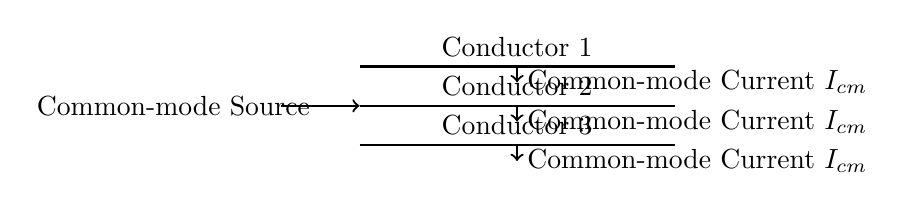
\begin{tikzpicture}
    % Draw the conductors
    \draw[thick] (0,1) -- (4,1) node[midway, above]{Conductor 1};
    \draw[thick] (0,0.5) -- (4,0.5) node[midway, above]{Conductor 2};
    \draw[thick] (0,0) -- (4,0) node[midway, above]{Conductor 3};

    % Add source
    \draw[->, thick] (-1,0.5) -- (0,0.5) node[midway, left]{Common-mode Source};

    % Indicate common-mode current direction
    \foreach \y in {1,0.5,0}{
        \draw[->, thick] (2,\y) -- (2,\y-0.2) node[below, right]{Common-mode Current $I_{cm}$};
    }
\end{tikzpicture}
